\chapter{Introduction}

\section{Supercomputing}

What do we mean by supercomputing? In general, we mean using computers to solve
problems which are very computationally intensive, i.e. problems which require
large computing resources in terms of memory or floating-point operations, or
both. Examples of problems requiring supercomputing are weather forecasting
(\url{http://met.no} uses the supercomputing facility here at NTNU), oil
exploration (reservoir simulation), seismic analysis (an inverse problem),
computational chemistry, computational physics, computational mechanics (e.g.
structural mechanics, fluid mechanics) and material science.

Due to the resource demanding aspects of supercomputing, it is important to make
the whole solution process as efficient as possible. Examples of important
issues to study are:
\begin{itemize}
\item numerical and computational algorithms which are fast, robust and accurate
\item software development
\item treatment of large data sets
\item visualization
\item validation of the simulation results
\end{itemize}
Supercomputing typically implies the use of parallel processing. This means that
the underlying algorithms used need to be designed and tuned for such a
computing environment. The software development typically becomes more involved
compared to a single-process implementation even though the trend is to abstract
the machine specific details as much as possible.

Because of the compute-intensive (memory, floating-point, I/O) nature of these
problems, they often require special high-end computing platforms. In Norway,
there is at least one such system at each major university. The large oil
companies in Norway also have such computing platforms. Each system is still
quite expensive to purchase, to operate and to maintain. In addition, special
intrastructure often needs to be built around such systems: special rooms
(security), power supply, cooling systems etc. Due to the overall investment,
both in terms hardware and in terms of human resources, it is important to use
these systems as efficiently as possible---each system typically lasts only a
few years.

Even if the current systems are powerful, it is important to make progress in
terms of making such systems easier to build and to use, and to develop more
efficient computational algorithms. This will enable larger and more realistic
problems to be simulated, which translates into progress in science and
engineering (which are the ``classical'' applications for supercomputing), but
also in other emerging areas such as the medical field.

In the following, let us briefly mention some of the issues involved when
working with a specific application. Assume that we have a program for
simulating the blood flow through part of a vein. Let $T_1$ be the solution time
on a single processor (even though, in reality, such a simulation would probably
not fit on a single-processor machine).

Assume now that we port this simulation to a multi-processor system with $P$
processors. Ideally, we would like the solution time to be reduced by a factor
of $P$. Another way of saying this is that we would like to achieve a speedup
\begin{align}
  S_p=T_1/T_p = P,
\end{align}
where $T_p$ is the solution time on $P$ processors. Typically, the speedup $S_p
< P$. As we increase the number of processors to solve our particular (fixed)
problem, we will first see a good speedup, followed by a degradation as we add
more and more processors. The main explanation for this is easy to understand.
In order to achieve a perfect speedup, we cannot have any overhead when moving
from a single processor system to a multi-processor system. In reality, we have
communication between the processors. As the number of processors is increased,
the work per processor goes down, while the overall communication overhead goes
up. A critical issue is therefore to minimize the communication overhead so that
we can take advantage of larger systems for a fixed problem.

We should here remark that one of the major advantages of having access to a
supercomputing facility is the possibility to solve much larger problems than
what is possible on a smaller system. Hence, as we increase the number of
processors, we may also increase the problem size so that the work per processor
remains fixed. We will consider some of these issues in this course.

Let us now discuss the single-processor performance a bit more. Assume for the
moment that we have two different versions (executables), $A$ and $B$, of a
particular application. We also assume that the underlying numerical algorithms
are identical. The simulation times for the two versions are denoted as $T_1^A$
and $T_1^B$, respectively. We observe that
\begin{align}
  T_1^A = 3 T_1^B.
\end{align}
Why are the two simulation times so different since the numerical algorithms are
the same?

\begin{figure}
  \centering
  \begin{tikzpicture}
    \matrix[
    column sep=4mm,
    every node/.style={
      shape=rectangle,
      rounded corners=1mm,
      draw=darkblue,
      fill=cadet,
      minimum height=1cm,
      text width=2.5cm,
      text centered,
      text height=1.5ex,
      text depth=.25ex,
    }]{
      \node (alg) {Algorithm}; &
      \node (prog) {Programming}; &
      \node (comp) {Compiler}; &
      \node (exe) {Executable}; \\
    };
    \begin{scope}[->, darkblue, thick]
      \draw (alg) -- (prog);
      \draw (prog) -- (comp);
      \draw (comp) -- (exe);
    \end{scope}
  \end{tikzpicture}
  \caption{Ingredients in a simulation.}
  \label{fig:single}
\end{figure}

We only mention a few aspects which may have caused this; see Figure \ref{fig:single}:
\begin{itemize}
\item different choice of data structure / memory layout during the programming;
\item different use of optimized numerical libraries;
\item different choices of compiler optimization.
\end{itemize}
We will look at some of these issues in this course.
Note that it is typically harder to achieve a good speedup for version B compared to
version A, even though $T_1^B  < T_1^A$ (can you suggest a reason why?)

Are there other ways to change the solution time for our particular simulation?
Yes; we mention two distinct ways:
\begin{itemize}
\item change the computer;
\item change the computational or numerical algorithms.
\end{itemize}
Progress in the available hardware has been impressive over the past decades.
However, it is important to realize that progress in computational algorithms
has been equally impressive. Note that developing a new algorithm which requires
only half the number of floating point operations is equally important as buying
a new computer with twice the performance in terms of floating point operations
per second (Flops).

We will discuss a few selected numerical algorithms in this course, e.g.
numerical solution of partial differential equations (primarily finite
difference methods), iterative and direct methods for solving linear systems of
equations, basic linear algebra routines, and a little bit about statistical
methods (Monte Carlo methods).

\section{Floating point representation}

This section gives a brief introduction to the IEEE standard (IEEE-754) for
floating point representation. A basic understanding of the standard is
appropriate given the importance of floating point operations in this course.

All real numbers are represented with a finite number of bits. The
representation is depicted in Figure \ref{fig:fp}. The sign bit is certainly
easy to understand. A value $S=0$ means that the number is positive, while a
value $S=1$ means that the number is negative.

\begin{figure}
  \centering
  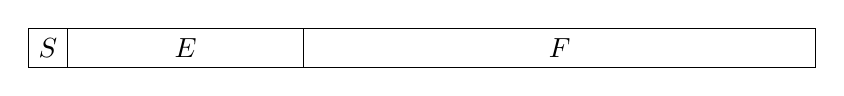
\begin{tikzpicture}[scale=0.5]
    \draw (0,0) rectangle (1,1);
    \draw (1,0) rectangle (7,1);
    \draw (7,0) rectangle (20,1);
    \node at (0.5, 0.5) {$S$};
    \node at (4, 0.5) {$E$};
    \node at (13.5, 0.5) {$F$};
  \end{tikzpicture}
  \caption{
    Each floating point has a binary representation with three fields: $S$
    denotes the sign of the number, $E$ is an exponent, and $F$ is the fraction
    part of the mantissa.
  }
  \label{fig:fp}
\end{figure}

The actual decimal value $V$ of the floating point is
\begin{align}
  V = (-1)^S \cdot 2^{E-B}\cdot M
\end{align}
where $M$ is the mantissa and $B$ is denoted as the \emph{bias} which will be
explained below. The exponent E is always adjusted such that the mantissa can be
expressed as
\begin{align}
  M = \underbrace{1}_{\times2^0} .
  \overbrace{\underbrace{b_1}_{\times2^{-1}}
  \underbrace{b_2}_{\times2^{-2}}\ldots}^{F}
\end{align}
where $F$ denotes the fraction of the mantissa in binary representation (i.e.
the binary digits $b_1b_2\ldots$). Since this representation is always assumed,
the binary number $1$ in the front is not explicitly represented. Note that,
\begin{align}
  1 \leq M < 2,
\end{align}
since the fraction $F$ is always less then one.

There are many more details regarding floating point representation. For
example, the implicitly assumed binary number 1 in the mantissa is only true for
what is referred to as {\em normalized} numbers.

\begin{table}
  \centering
  \caption{Number of bits for common floating point standards.}
  \bgroup\def\arraystretch{1.2}
  \begin{tabular}{ccccc} \hline
    Precision & $S$ & $E$ & $F$ & Total \\ \hhline{=====}
    Single & $1$ & $8$ & $23$ & 32
    \\ \hline
    Double & $1$ & $11$ & $52$ & 64
    \\ \hline
  \end{tabular}
  \egroup
\end{table}

A few words about the exponent $E$. In single precision, $E$ is represented
using 8 bits, giving 256 possibilities, of which 254 are used to represent
normalized numbers. The values $E=0$ and $E=255$ are primarily reserved for zero
and infinities. The actual exponent used to find the corresponding decimal value
of a normalized number is $E-B$; see equation (1). For single precision,
$B=127$ and for double precision, $B=1023$.

We can now compute the maximum and minimum numbers that we can represent in
single precision (i.e. using 32 bits):
\begin{alignat}{2}
  \label{maxnumber}
  V_{\text{max}} &= 1 \cdot 2^{254-127} \cdot 2 &&\approx 3.40 \cdot 10^{38} \\
  \label{minnumber}
  V_{\text{min}} &= 1\cdot 2^{1-127} \cdot 1 &&\approx 1.17 \cdot 10^{-38}
\end{alignat}
As we can see, this is a significant range.

Having considered the range, let us now consider the accuracy of a given
floating point number. Again, consider the single precision case. The fraction
of the mantissa is represented using 23 bits, meaning that the smallest {\em
fraction} that can be represented is
\begin{align*}
  2^{-23} \approx 1.19 \cdot 10^{-7}.
\end{align*}
This implies that {\em any} floating point number using single precision
(covering the whole range discussed above) has about 7 digits of accuracy.

\begin{ex}
  Consider the maximum and minimum numbers defived in
  \eqref{maxnumber}-\eqref{minnumber}. How many digits should we include in each
  of these numbers when written out?
\end{ex}

\begin{ex}
  Find the binary floating point representation of the decimal number $4.25$ in
  single precision.
\end{ex}

\begin{ex}
  How many decimal digits of accuracy does a double precision floating point
  number have?
\end{ex}

\section{Integer representation}

An integer is typically represented using 32 bits. One bit is used to represent
the sign. Hence, the possible integers will be in the range $\pm 2^{31} \approx
\pm 2\cdot 10^9$.

If an algorithm includes a loop which needs to be done $n$ times (e.g., a Monte
Carlo simulation), $n$ needs to be less than approximately $10^9$. This may seem
sufficient, however, there could be situations when this limitation could become
an issue.

\begin{ex}
  Propose one or several ways around this limitation.
\end{ex}

\section{Floating point performance}

The basic operations of adding, multiplying, subtracting and dividing two
floating point numbers are counted as floating point operations.

Floating point performance is usually measured in number of floating point
operations per second, commonly abbreviated as Flops; for a brief discussion
see \url{http://en.wikipedia.org/wiki/FLOPS}.

Since current computer systems typically perform many of these operations per
seconds, abbreviations like MFlops (megaflops), GFlops (gigaflops), TFlops
(teraflops), and PFlops (petaflops) are common to use.

When we speak about the speed of a computer, we will typically mean the floating
point performance.

\begin{ex}
  Let $c$ be a scalar (a floating point number), let $\bm x$, $\bm y$, and $\bm
  z$ be vectors, each comprising $n$ floating point numbers, and let $\bm A$ be
  an $n\times n$ matrix. How many floating point operations does it take to
  perform the following basic linear algebra operations?
  \begin{align*}
  \bm z = \bm x + c \bm y, \qquad \bm y = \bm A \bm x
  \end{align*}
\end{ex}

\section{Storage requirements}

It is quite common today to do all the necessary computations using double
precision. This means that 64 bits are used to represent each floating point
number, which is equivalent to 8 bytes (8 bits per byte).

Let us now consider how many floating point numbers we can store in the memory
associated with a typical processor. Assume that we have available
$\SI{4}{\giga\byte}$ ($4\cdot 10^9$ bytes) of main memory (or RAM: \emph{Random
Access Memory}); this is a quite typical size nowadays. This amount of memory is
sufficient to represent a total of 512 millon floating point numbers in double
precision.

In practice, we could never use the entire memory for such a purpose. We also
need space for our simulation program (instructions etc.). However, it gives an
indication of the order of magnitude that we can handle.

If we are solving differential equations or some other problem, we also need to
use memory to store matrices, temporary variables, etc. The available memory to
store the actual solution depends on the numerical algorithm, however even a
fairly scalable algorithm would typically only be able to handle a few million
unknowns. Many algorithms would allow far fewer unknowns.

Problems in science and engineering can easily require many million unknowns,
perhaps even billions of unknowns. In order to solve such problems, we obviously
need both more memory and increased computing power. This is achieved using
parallel processing where multiple processors and memory modules are connected
into a single computational platform.

\begin{ex}
  Let $\bm A$ be an $n\times n$ matrix, and $\bm x$ and $\bm b$ be two vectors
  of length $n$. Assume that we want to solve the linear system of equations
  \begin{align*}
    \bm A \bm x = \bm b
  \end{align*}
  using Gaussian elimination. Assume further that the matrix $\bm A$ is dense,
  meaning that we need to store all the $n^2$ entries in the matrix.

  What is (approximately) the largest equation system we can solve (i.e., the
  largest number of $n$ we can use) and still be able to fit the whole problem
  in the main memory, which we assume is $\SI{1}{\giga\byte}$?
\end{ex}

\section{Past, current and future supercomputers}

\autoref{fig:perform-dev} depicts the past and future performance development
of the 500 fastest supercomputers in the world. More information about the top
500 systems can be found on \url{http://top500.org}.

In 1986 a supercomputing center was established at NTH.
\autoref{tab:history-ntnu} gives a summary of the supercomputers at NTH/NTNU
since then.

\begin{figure}
  \centering
  \begin{tikzpicture}
    \begin{axis}[
      date coordinates in=x,
      ymode=log,
      xticklabel=\year,
      xmin=1993-05-01,
      xmax=2015-10-01,
      width=\textwidth,
      height=0.4\textheight,
      ytick={1, 1000, 1000000, 1000000000},
      yticklabels={$\SI{1}{\giga\flop}$, $\SI{1}{\tera\flop}$, $\SI{1}{\peta\flop}$, $\SI{1}{\exa\flop}$},
      grid=major,
      legend style={at={(1,0)}, anchor=south east},
      legend cell align=left,
      ]
      \addplot[mark=o, mark size=1.3, draw=darkgreen, thick]
      table[x=date, y=sum, col sep=comma]
      {data/performance-development.csv};
      \addplot[mark=o, mark size=1.3, draw=red, thick]
      table[x=date, y=high, col sep=comma]
      {data/performance-development.csv};
      \addplot[mark=o, mark size=1.3, draw=magenta, thick]
      table[x=date, y=low, col sep=comma]
      {data/performance-development.csv};
      \legend{Sum, Highest, Lowest};
    \end{axis}
  \end{tikzpicture}
  \caption{
    The performance development since 1993 for the top 500 supercomputers in the
    world. In particular, the figure indicates the performance development for
    the fastest system (number 1), the slowest system (number 500), and the sum
    of all the 500 fastest systems.
  }
  \label{fig:perform-dev}
\end{figure}

\begin{table}
  \caption{
    Supercomputers at NTH/NTNU. Note that some of this information is guesswork
    as not all machines were not available at when revising this document.
  }
  \centering
  \bgroup\def\arraystretch{1.2}
  \begin{tabular}{llrlr}
    \hline
    Year & System & Processors & Type & GF\footnote{maximal theoretical performance in $\SI{}{\giga\flop}$} \\
    \hhline{=====}
    1986--1992 & Cray X-MP & 2 & Vector & 0.5 \\
    1992--1996 & Cray Y-MP & 4 & Vector & 1.3\\
    1995--2003 & Cray J90     & 8 & Vector & 1.6 \\
    1992--1999 & Intel Paragon & 56 & MPP & 5.0\\
    1996--2003 & Cray T3E & 96 & MPP & 58\\
    2000--2001 & SGI O2 & 160 & ccNUMA & 100\\
    2001--2008 & SGI O3 & 898 & ccNUMA & 1000\\
    2006--2011 & IBM P5+ & 2976 & Distributed SMP & 23500\\
    2012--     & SGI Altix ICE X & 23040 & Distributed SMP & 497230 \\
    \hline
  \end{tabular}
  \egroup
  \label{tab:history-ntnu}
\end{table}

The current supercomputer at NTNU is an SGI Altix system with 20736 (physical)
processors. For an example of what such a system looks like, see
\autoref{fig:njord}. Some of the exercises in this course will be done using
this system. Some of the key characteristics of this system are:
\begin{itemize}
\item Full name: \texttt{vilje.hpc.ntnu.no}
\item System: SGI Altix ICE
\item Type: Distributed SMP
\item Number of nodes: 1440
\item Nodes: Shared memory system; 2 octa-core chips; 32 GB memory
\item Number of cores (processors): 23040
\item CPU type: Intel Sandy Bridge
\item Theoretical peak performance: 479.23 TFlops
\item Weight: This machine is shy and refuses to tell me
\end{itemize}

\begin{figure}
  \centering
  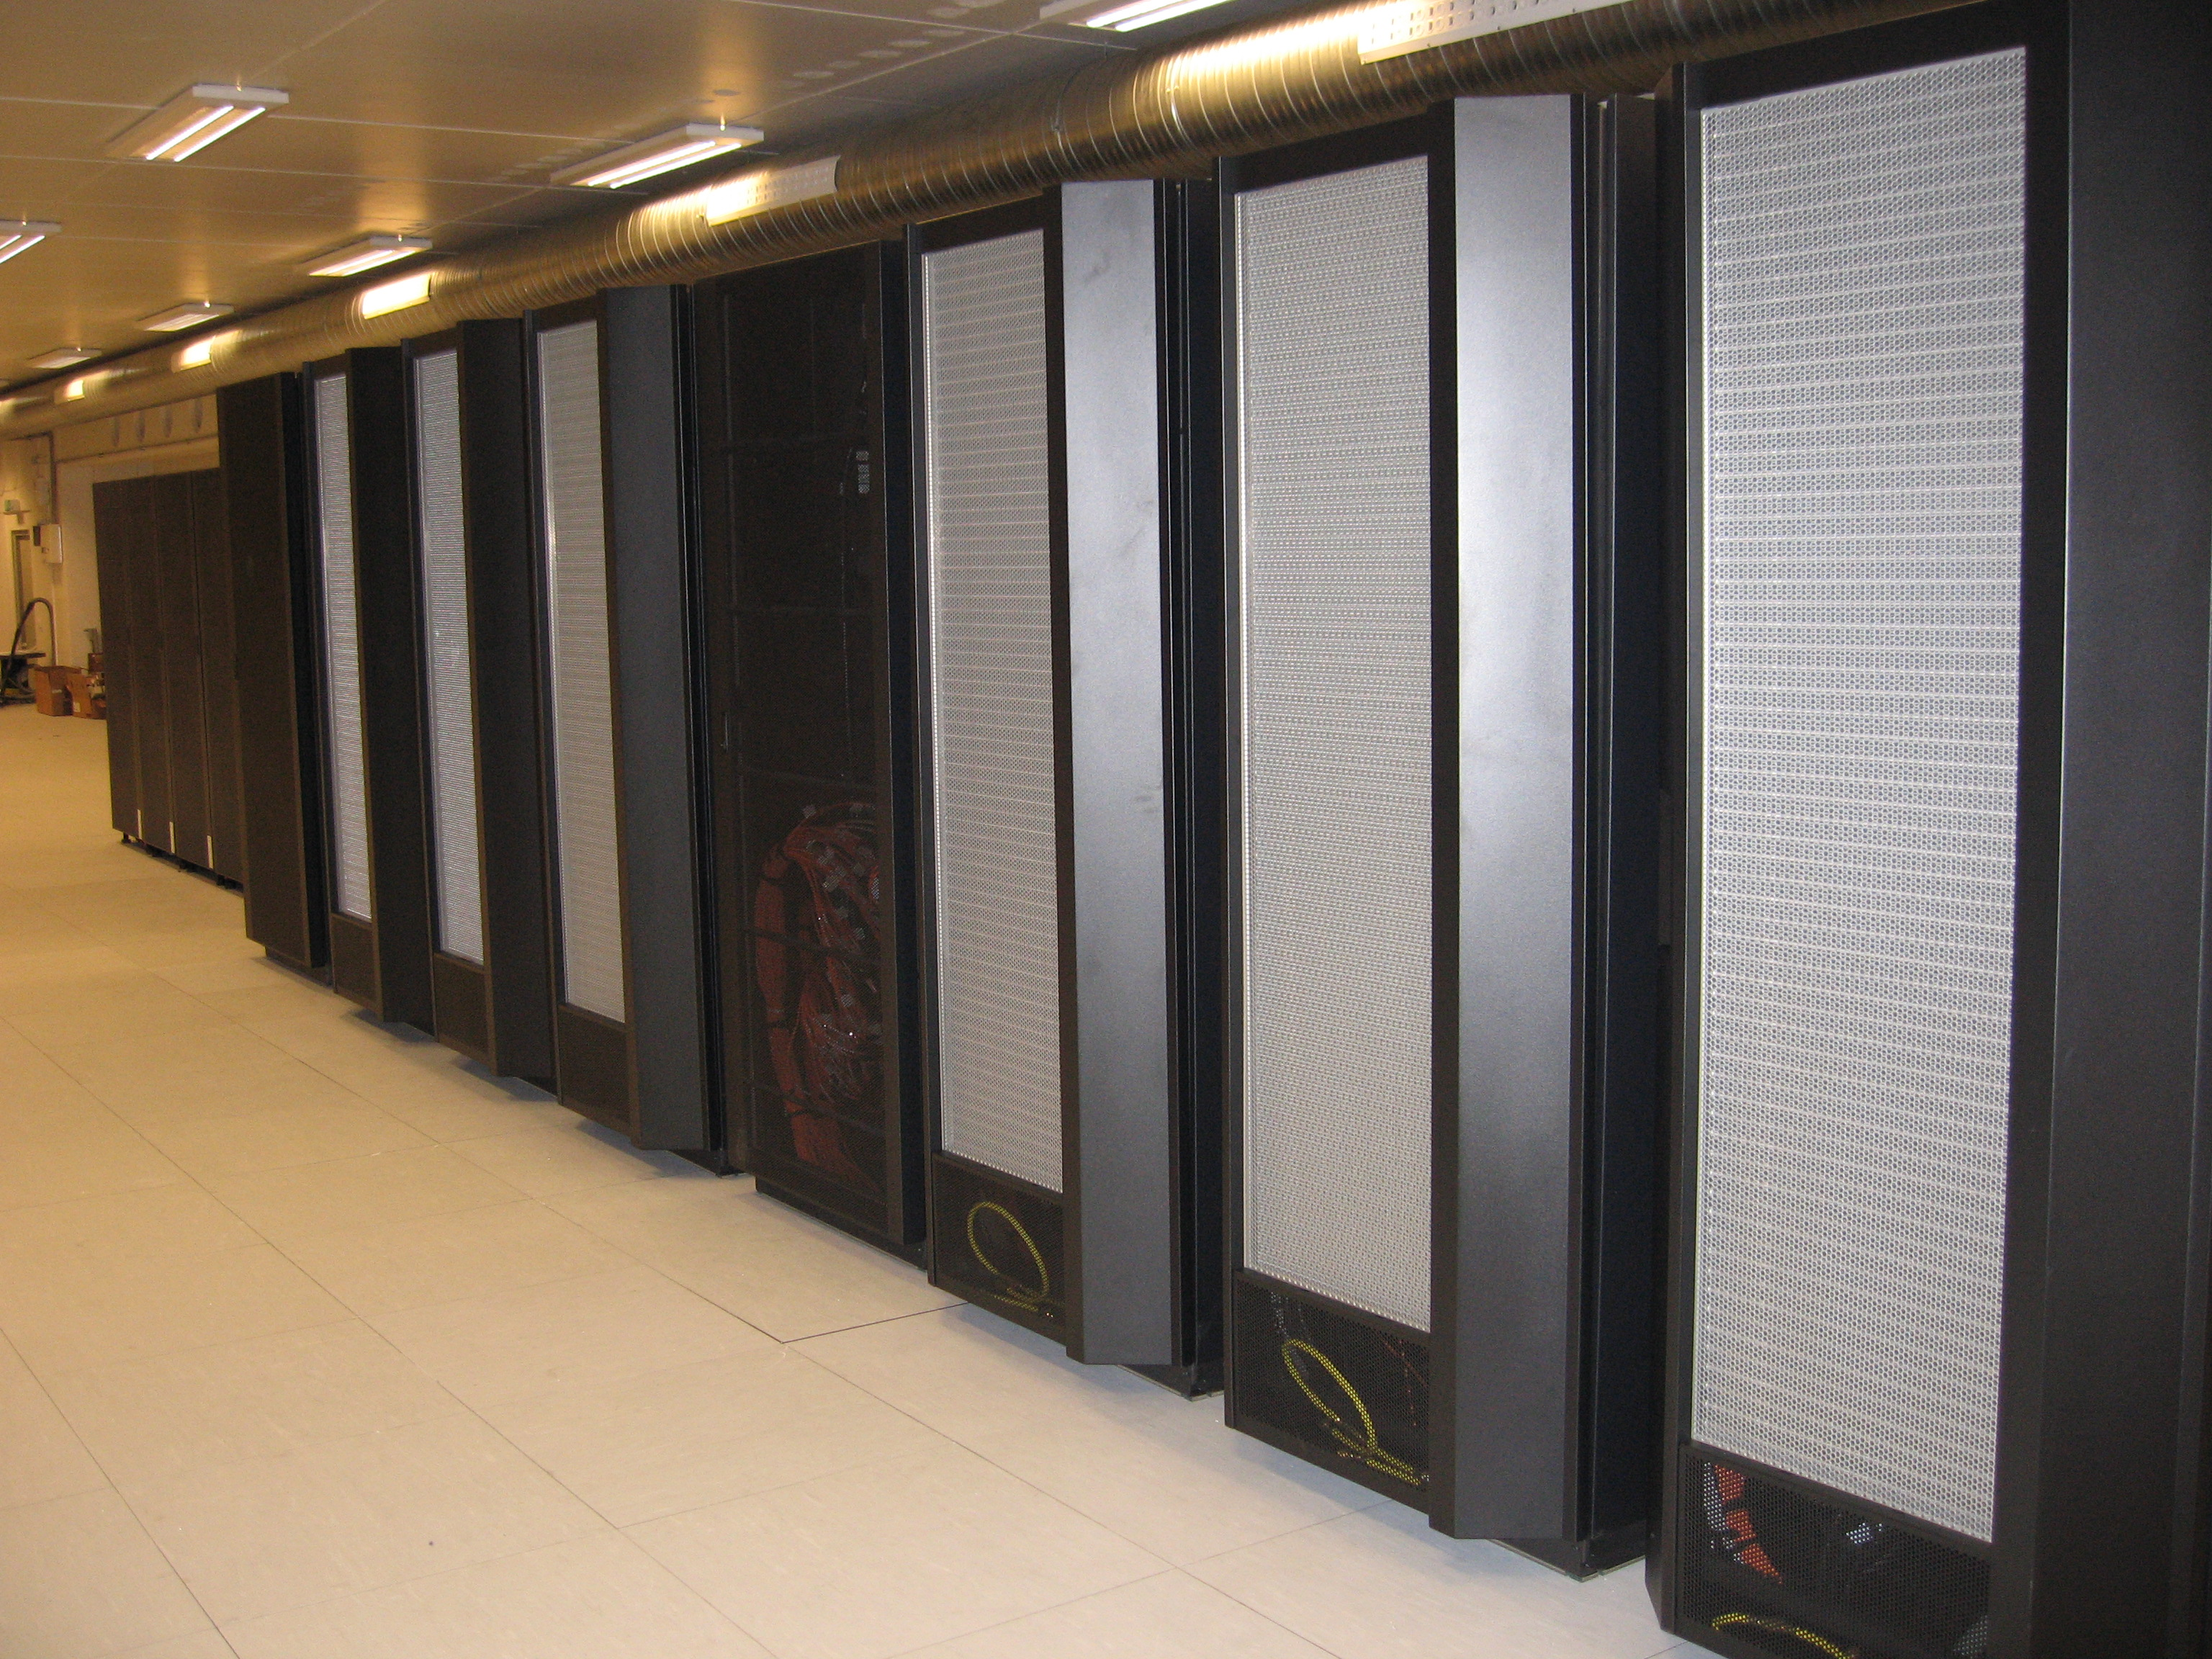
\includegraphics[width=0.6\textwidth]{njord_2}
  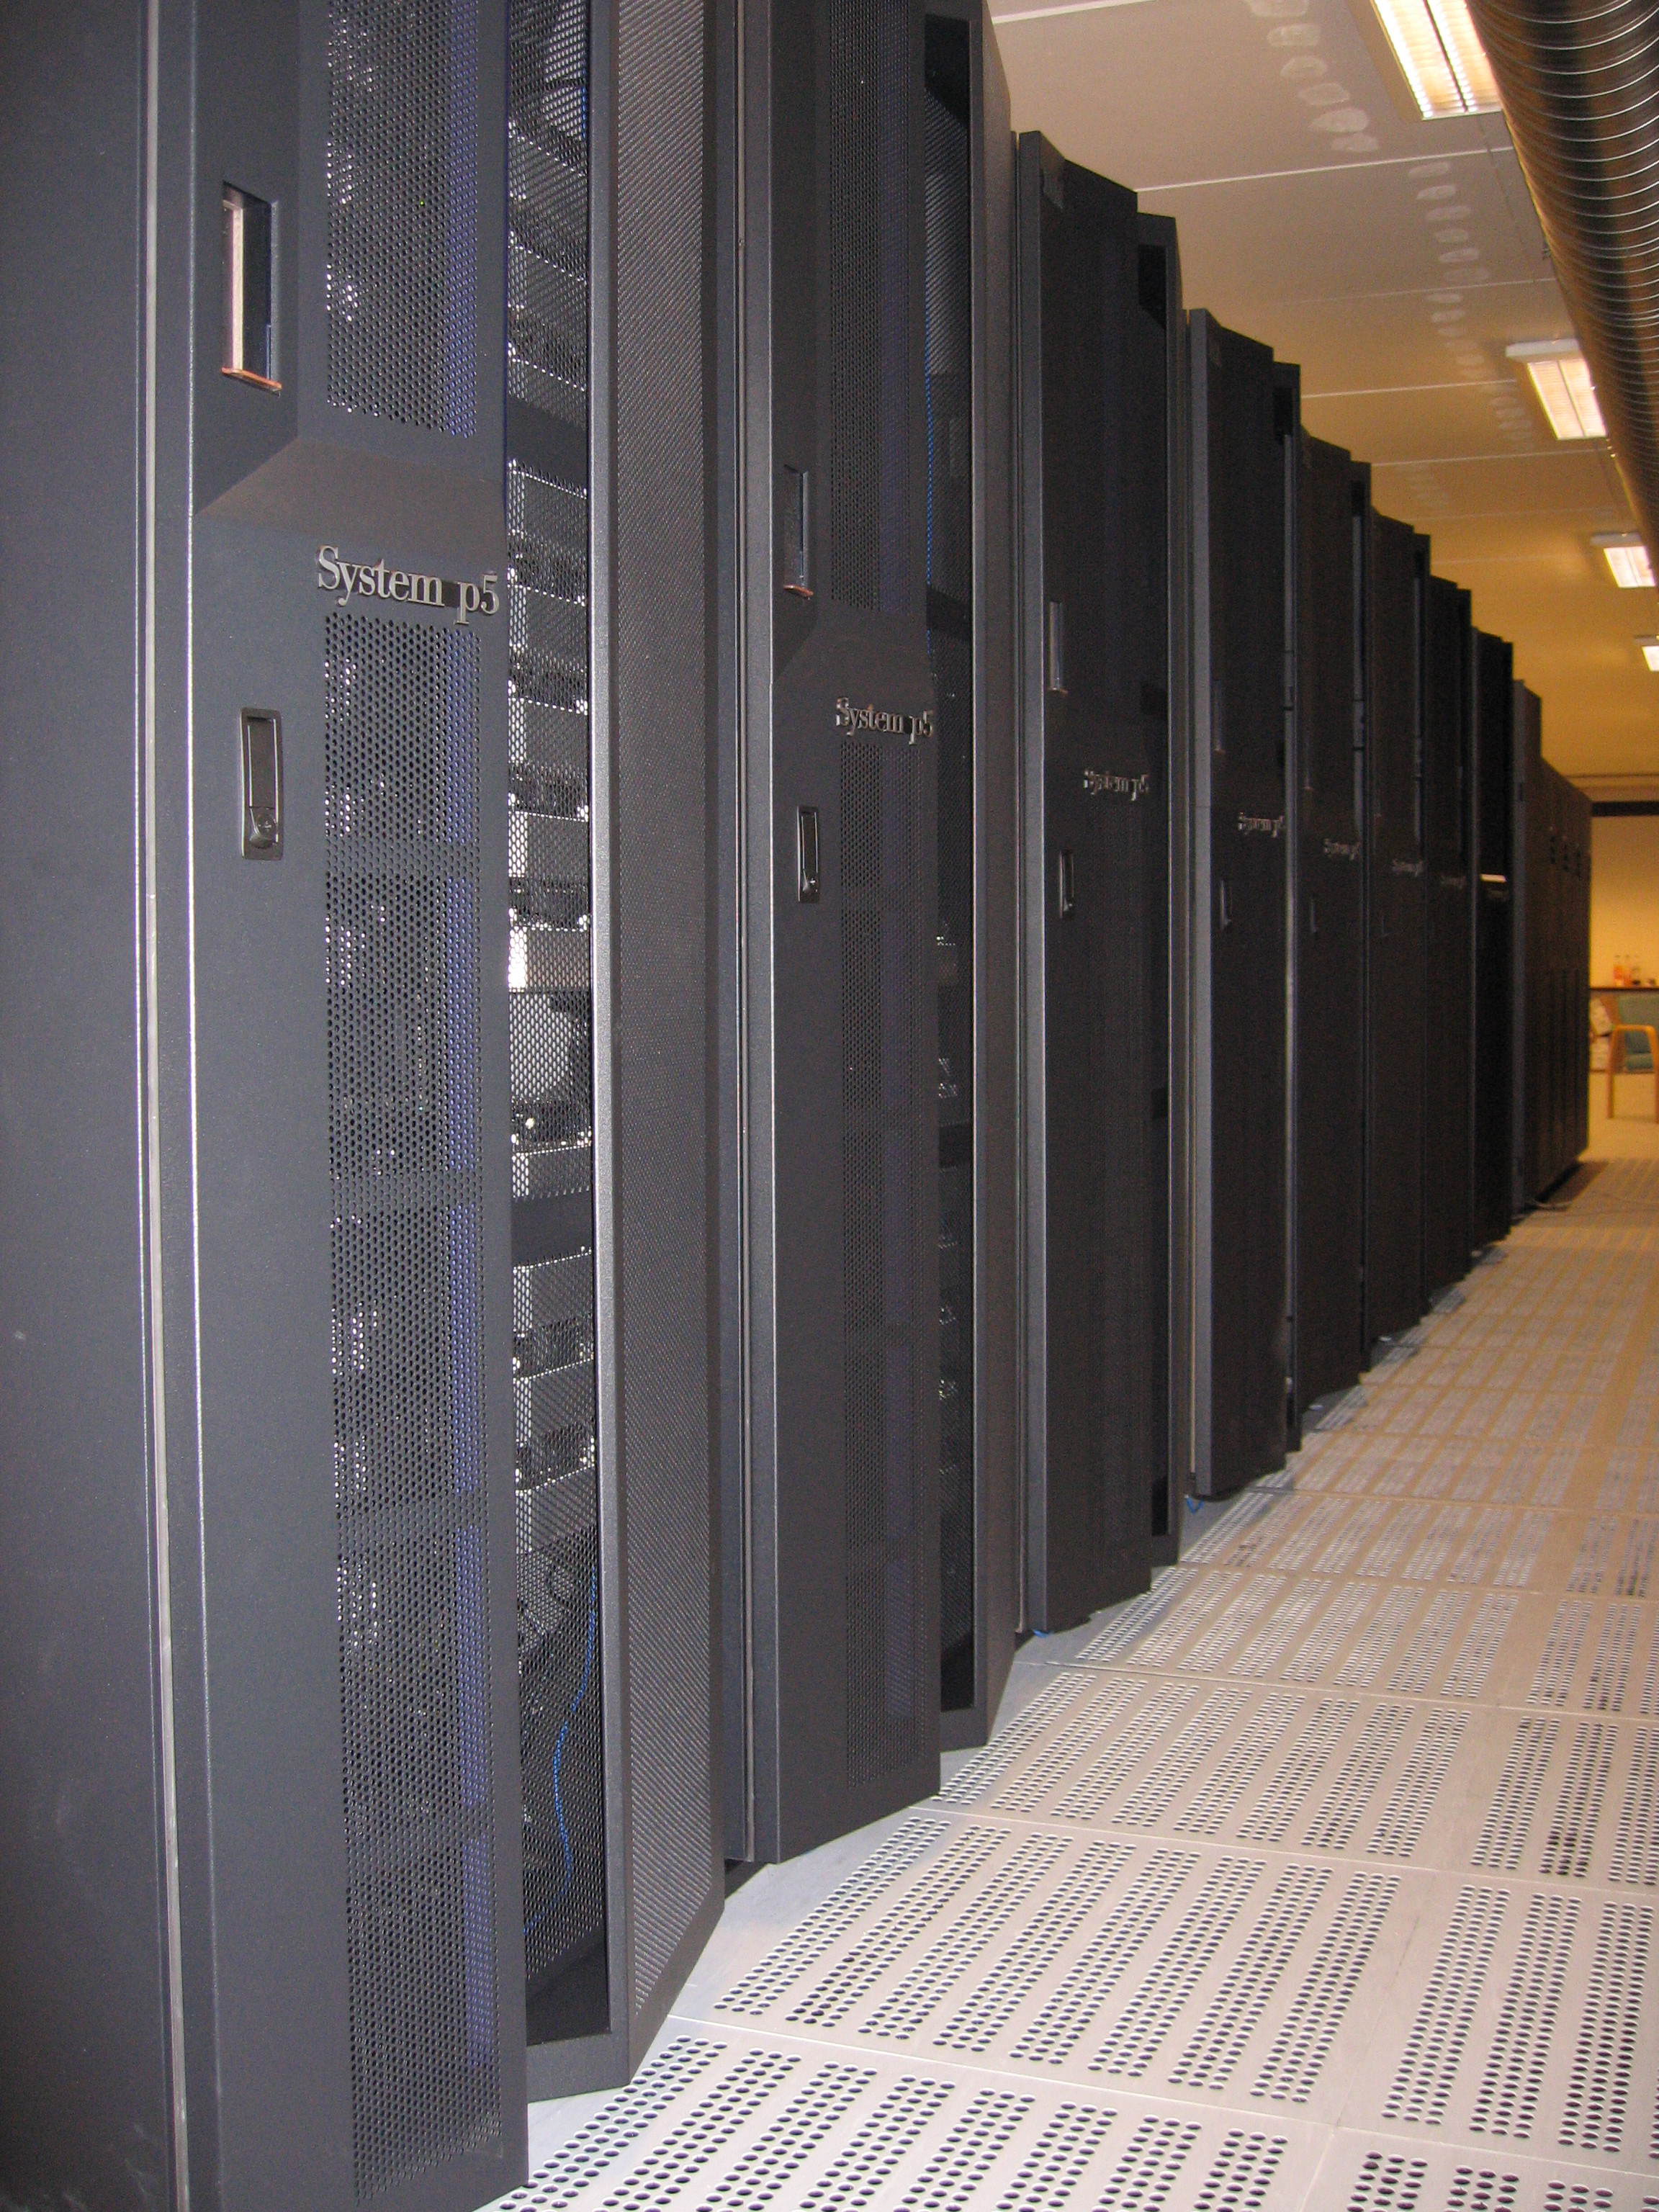
\includegraphics[width=0.6\textwidth]{njord_1}
  \caption{
    Photos of \emph{Njord}, the previous IBM supercomputer system at NTNU.
    Courtesy of Arve Dispen.
  }
  \label{fig:njord}
\end{figure}

\section{Applications}

Some sample applications for supercomputing are given in \Autoref{fig:met,
fig:climate}.

\vspace{2cm}
\begin{figure}[!ht]
  \centering
  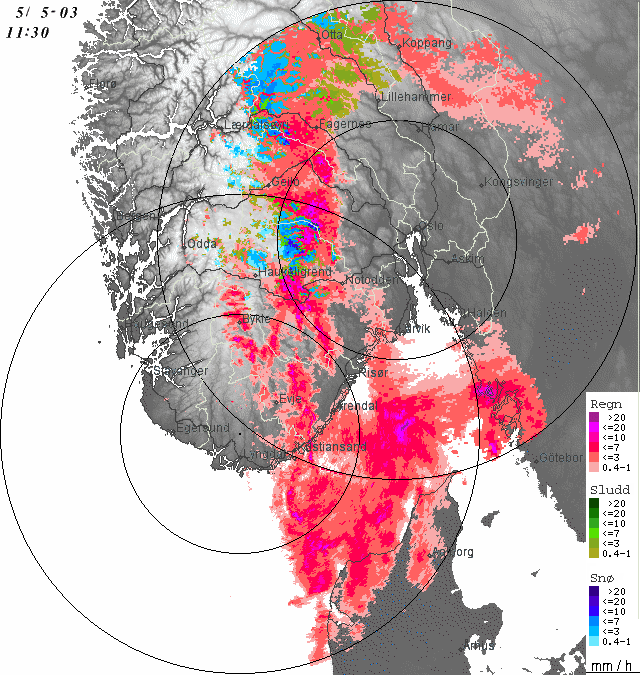
\includegraphics[height=0.6\textheight]{met}
  \caption{
    Example of use of supercomputing: weather forecasting. The Meteorological
    Institute in Norway uses the supercomputer \emph{Njord} every day. Source:
    \protect\url{http://met.no}.
  }
  \label{fig:met}
\end{figure}

\begin{figure}[!ht]
  \centering
  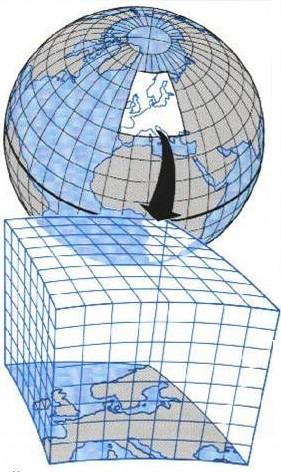
\includegraphics[height=0.6\textheight]{climate_model}
  \caption{
    Example of use of supercomputing: climate modelling. For more information,
    see \protect\url{http://bjerknes.uib.no} (Bjerknes Centre for Climate Research).
  }
  \label{fig:climate}
\end{figure}
